% Created by tikzDevice version 0.12.3.1 on 2021-12-06 10:55:34
% !TEX encoding = UTF-8 Unicode
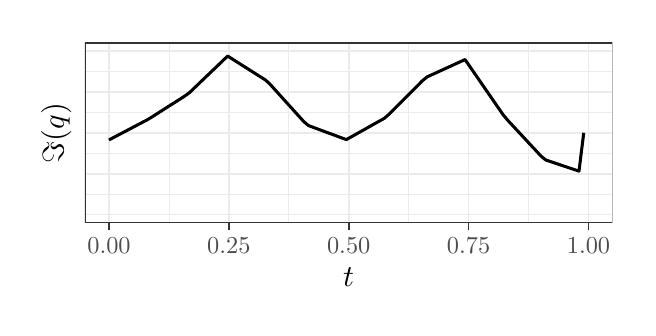
\begin{tikzpicture}[x=1pt,y=1pt]
\definecolor{fillColor}{RGB}{255,255,255}
\path[use as bounding box,fill=fillColor,fill opacity=0.00] (0,0) rectangle (216.81,101.18);
\begin{scope}
\path[clip] (  0.00,  0.00) rectangle (216.81,101.18);
\definecolor{drawColor}{RGB}{255,255,255}
\definecolor{fillColor}{RGB}{255,255,255}

\path[draw=drawColor,line width= 0.6pt,line join=round,line cap=round,fill=fillColor] (  0.00,  0.00) rectangle (216.81,101.18);
\end{scope}
\begin{scope}
\path[clip] ( 20.71, 30.69) rectangle (211.31, 95.68);
\definecolor{fillColor}{RGB}{255,255,255}

\path[fill=fillColor] ( 20.71, 30.69) rectangle (211.31, 95.68);
\definecolor{drawColor}{gray}{0.92}

\path[draw=drawColor,line width= 0.3pt,line join=round] ( 20.71, 41.03) --
	(211.31, 41.03);

\path[draw=drawColor,line width= 0.3pt,line join=round] ( 20.71, 55.80) --
	(211.31, 55.80);

\path[draw=drawColor,line width= 0.3pt,line join=round] ( 20.71, 70.57) --
	(211.31, 70.57);

\path[draw=drawColor,line width= 0.3pt,line join=round] ( 20.71, 85.34) --
	(211.31, 85.34);

\path[draw=drawColor,line width= 0.3pt,line join=round] ( 51.04, 30.69) --
	( 51.04, 95.68);

\path[draw=drawColor,line width= 0.3pt,line join=round] ( 94.35, 30.69) --
	( 94.35, 95.68);

\path[draw=drawColor,line width= 0.3pt,line join=round] (137.67, 30.69) --
	(137.67, 95.68);

\path[draw=drawColor,line width= 0.3pt,line join=round] (180.99, 30.69) --
	(180.99, 95.68);

\path[draw=drawColor,line width= 0.6pt,line join=round] ( 20.71, 33.64) --
	(211.31, 33.64);

\path[draw=drawColor,line width= 0.6pt,line join=round] ( 20.71, 48.41) --
	(211.31, 48.41);

\path[draw=drawColor,line width= 0.6pt,line join=round] ( 20.71, 63.18) --
	(211.31, 63.18);

\path[draw=drawColor,line width= 0.6pt,line join=round] ( 20.71, 77.95) --
	(211.31, 77.95);

\path[draw=drawColor,line width= 0.6pt,line join=round] ( 20.71, 92.72) --
	(211.31, 92.72);

\path[draw=drawColor,line width= 0.6pt,line join=round] ( 29.38, 30.69) --
	( 29.38, 95.68);

\path[draw=drawColor,line width= 0.6pt,line join=round] ( 72.69, 30.69) --
	( 72.69, 95.68);

\path[draw=drawColor,line width= 0.6pt,line join=round] (116.01, 30.69) --
	(116.01, 95.68);

\path[draw=drawColor,line width= 0.6pt,line join=round] (159.33, 30.69) --
	(159.33, 95.68);

\path[draw=drawColor,line width= 0.6pt,line join=round] (202.65, 30.69) --
	(202.65, 95.68);
\definecolor{drawColor}{RGB}{0,0,0}

\path[draw=drawColor,line width= 1.1pt,line join=round] ( 29.38, 60.61) --
	( 31.09, 61.52) --
	( 32.81, 62.42) --
	( 34.52, 63.32) --
	( 36.24, 64.22) --
	( 37.96, 65.13) --
	( 39.67, 66.03) --
	( 41.39, 66.93) --
	( 43.10, 67.83) --
	( 44.82, 68.86) --
	( 46.53, 69.95) --
	( 48.25, 71.05) --
	( 49.96, 72.14) --
	( 51.68, 73.23) --
	( 53.40, 74.32) --
	( 55.11, 75.41) --
	( 56.83, 76.51) --
	( 58.54, 77.78) --
	( 60.26, 79.42) --
	( 61.97, 81.07) --
	( 63.69, 82.71) --
	( 65.40, 84.35) --
	( 67.12, 85.99) --
	( 68.84, 87.63) --
	( 70.55, 89.28) --
	( 72.27, 90.92) --
	( 73.98, 89.83) --
	( 75.70, 88.75) --
	( 77.41, 87.66) --
	( 79.13, 86.58) --
	( 80.84, 85.49) --
	( 82.56, 84.40) --
	( 84.27, 83.32) --
	( 85.99, 82.23) --
	( 87.71, 80.60) --
	( 89.42, 78.70) --
	( 91.14, 76.80) --
	( 92.85, 74.90) --
	( 94.57, 73.00) --
	( 96.28, 71.10) --
	( 98.00, 69.20) --
	( 99.71, 67.30) --
	(101.43, 65.82) --
	(103.15, 65.18) --
	(104.86, 64.54) --
	(106.58, 63.91) --
	(108.29, 63.27) --
	(110.01, 62.64) --
	(111.72, 62.00) --
	(113.44, 61.36) --
	(115.15, 60.73) --
	(116.87, 61.69) --
	(118.59, 62.65) --
	(120.30, 63.62) --
	(122.02, 64.58) --
	(123.73, 65.54) --
	(125.45, 66.51) --
	(127.16, 67.47) --
	(128.88, 68.43) --
	(130.59, 69.90) --
	(132.31, 71.63) --
	(134.03, 73.35) --
	(135.74, 75.07) --
	(137.46, 76.80) --
	(139.17, 78.52) --
	(140.89, 80.25) --
	(142.60, 81.97) --
	(144.32, 83.38) --
	(146.03, 84.17) --
	(147.75, 84.95) --
	(149.47, 85.74) --
	(151.18, 86.52) --
	(152.90, 87.30) --
	(154.61, 88.09) --
	(156.33, 88.87) --
	(158.04, 89.66) --
	(159.76, 87.17) --
	(161.47, 84.68) --
	(163.19, 82.19) --
	(164.90, 79.71) --
	(166.62, 77.22) --
	(168.34, 74.73) --
	(170.05, 72.24) --
	(171.77, 69.76) --
	(173.48, 67.70) --
	(175.20, 65.85) --
	(176.91, 64.01) --
	(178.63, 62.16) --
	(180.34, 60.32) --
	(182.06, 58.47) --
	(183.78, 56.63) --
	(185.49, 54.78) --
	(187.21, 53.36) --
	(188.92, 52.79) --
	(190.64, 52.21) --
	(192.35, 51.64) --
	(194.07, 51.06) --
	(195.78, 50.49) --
	(197.50, 49.91) --
	(199.22, 49.34) --
	(200.93, 63.18);
\definecolor{drawColor}{gray}{0.20}

\path[draw=drawColor,line width= 0.6pt,line join=round,line cap=round] ( 20.71, 30.69) rectangle (211.31, 95.68);
\end{scope}
\begin{scope}
\path[clip] (  0.00,  0.00) rectangle (216.81,101.18);
\definecolor{drawColor}{gray}{0.20}

\path[draw=drawColor,line width= 0.6pt,line join=round] ( 29.38, 27.94) --
	( 29.38, 30.69);

\path[draw=drawColor,line width= 0.6pt,line join=round] ( 72.69, 27.94) --
	( 72.69, 30.69);

\path[draw=drawColor,line width= 0.6pt,line join=round] (116.01, 27.94) --
	(116.01, 30.69);

\path[draw=drawColor,line width= 0.6pt,line join=round] (159.33, 27.94) --
	(159.33, 30.69);

\path[draw=drawColor,line width= 0.6pt,line join=round] (202.65, 27.94) --
	(202.65, 30.69);
\end{scope}
\begin{scope}
\path[clip] (  0.00,  0.00) rectangle (216.81,101.18);
\definecolor{drawColor}{gray}{0.30}

\node[text=drawColor,anchor=base,inner sep=0pt, outer sep=0pt, scale=  0.88] at ( 29.38, 19.68) {0.00};

\node[text=drawColor,anchor=base,inner sep=0pt, outer sep=0pt, scale=  0.88] at ( 72.69, 19.68) {0.25};

\node[text=drawColor,anchor=base,inner sep=0pt, outer sep=0pt, scale=  0.88] at (116.01, 19.68) {0.50};

\node[text=drawColor,anchor=base,inner sep=0pt, outer sep=0pt, scale=  0.88] at (159.33, 19.68) {0.75};

\node[text=drawColor,anchor=base,inner sep=0pt, outer sep=0pt, scale=  0.88] at (202.65, 19.68) {1.00};
\end{scope}
\begin{scope}
\path[clip] (  0.00,  0.00) rectangle (216.81,101.18);
\definecolor{drawColor}{RGB}{0,0,0}

\node[text=drawColor,anchor=base,inner sep=0pt, outer sep=0pt, scale=  1.10] at (116.01,  7.64) {$t$};
\end{scope}
\begin{scope}
\path[clip] (  0.00,  0.00) rectangle (216.81,101.18);
\definecolor{drawColor}{RGB}{0,0,0}

\node[text=drawColor,rotate= 90.00,anchor=base,inner sep=0pt, outer sep=0pt, scale=  1.10] at ( 13.08, 63.18) {$\Im(q)$};
\end{scope}
\end{tikzpicture}
